% This file is for creating and tweaking one plot at a time. When working on one plot, we don't want
% to do that in the context of a document that contains a lot of other stuff because that makes the
% edit -> compile -> inspect cycle very long. We create and tweak the plot here and once it's
% finished, we move the code over into another place like DemoPlots.tex.

%\documentclass[12pt, twocolumn]{article}
%\documentclass[12pt, openany]{book}
\documentclass[12pt, oneside]{book}
%\usepackage{fullpage}           % makes all margins 1 inch?
\topmargin=-1.0cm
\textheight=23cm
\evensidemargin=-1.0cm
\oddsidemargin=-1.0cm
\textwidth=19cm
\setcounter{secnumdepth}{-1}  % suppress numbering of sections
\usepackage{amsmath}
\usepackage{amssymb}          % for mathbb
\usepackage{hyperref}
\usepackage{array}            % For Cayley tables
\usepackage{stmaryrd}         % for \llbracket, \rrbracket
%\usepackage{cancel}           % \cancel to strike out math symbols - nah - it's ugly

\usepackage{comment}          
% to comment out larger sections via \begin{comment} ... \end{comment} 
% see:
% https://tex.stackexchange.com/questions/17816/commenting-out-large-sections
% https://tex.stackexchange.com/questions/11177/how-to-write-hidden-notes-in-a-latex-file/73418


\usepackage{color}               % colored text
\usepackage{listings}            % source code formatting 
%\lstset{language=python}
\definecolor{mygreen}{rgb}{0,0.6,0}
\definecolor{mygray}{rgb}{0.5,0.5,0.5}
\definecolor{mymauve}{rgb}{0.58,0,0.82}
\lstset{ %
  backgroundcolor=\color{white},   
  %basicstyle=\footnotesize\ttfamily,  % the size of the fonts that are used for the code
  basicstyle=\ttfamily,               % the size of the fonts that are used for the code
  captionpos=none,                    % no captions (and no empty space either)
  commentstyle=\color{mygreen},       % comment style
  frame=single,	                      % adds a frame around the code
  keywordstyle=\color{blue},          % keyword style
  language=Python,
  stringstyle=\color{mymauve},        % string literal style
  columns=flexible,                   %
  keepspaces=true,                    % keeps spaces in text
  tabsize=4,
}


\usepackage{tikz}
%\usetikzlibrary{calc} % maybe later
\usetikzlibrary{positioning}


\usepackage{mathtools}                        % for "\DeclarePairedDelimiter" macro

% Constants:
\DeclareMathOperator{\e}{\mathrm{e}}          % for Euler's number - ToDo: use \e consistently!
%\newcommand{\e}{\operatorname{e}}            % ...alternative definition (possibly)

% Functions:
\DeclareMathOperator{\li}{li}                      % Integral logarithm
\DeclareMathOperator{\Li}{Li}                      % Integral logarithm
\DeclareMathOperator{\sign}{sign}    
\DeclareMathOperator{\atan2}{atan2}
\DeclarePairedDelimiter{\floor}{\lfloor}{\rfloor}
\newcommand{\norm}[1]{\left\lVert#1\right\rVert}   % different norms?

% Matrix stuff:
\DeclareMathOperator{\rank}{rank}             % rank
\DeclareMathOperator{\vectorize}{vec}         % matrix to vector (concat columns)
\DeclareMathOperator{\tr}{tr}                 % trace
\DeclareMathOperator{\geo}{geo}               % geometric multiplicity
\DeclareMathOperator{\alg}{alg}               % algebraic multiplicity 

% Multivariable calculus:
%\DeclareMathOperator{\d}{d}                  % exterior derivative
\DeclareMathOperator{\grad}{\mathbf{grad}}
\DeclareMathOperator{\curl}{\mathbf{curl}}
\DeclareMathOperator{\dive}{div}

% Set theory:
\DeclareMathOperator{\im}{im}                 % image of a function/map
\DeclareMathOperator{\card}{card}             % cardinality        
\DeclareMathOperator{\tc}{tc}                 % transitive closure of a set
%\DeclareMathOperator{\Eig}{Eig} 

% Logic:
% There are multiple conventions to express a logical exclusive or - we make the choice for the
% whole text here:
\newcommand*\xor{\mathbin{\veebar}}              % exclusive or - alternatives: \oplus, \dot{\vee}
\newcommand*\nand{\mathbin{\barwedge}}
\newcommand*\then{\mathbin{\rightarrow}}         % \implies is already defined
\newcommand*\mequiv{\mathbin{\leftrightarrow}}   % material equivalence
% We follow wolfram:
% https://mathworld.wolfram.com/XOR.html
% https://mathworld.wolfram.com/NAND.html

%\let\cleardoublepage\clearpage

% Maybe move the stuff up to here into a _Setup.tex file that can be included from
% _FullBook.tex and _SingleChapter.tex

% These two lines will show the preview picture on a page that is adapted to the size of the pic:
%\usepackage[active,tightpage]{preview}
%\PreviewEnvironment{tikzpicture}


\begin{document}


\begin{figure}[h]
\centering

% The numbers in the comment behind the plot give a good setting for width, height, i.e. 18,15 means
% that the plot looks good when using "\pgfplotsset{width=18cm,height=15cm}", for example. 18,12..15
% gives a range of 12 to 15 for the height

\pgfplotsset{width=18cm,height=12cm}

% Finished plots:
%\pgfplotsset{compat=1.18}

\begin{tikzpicture}[thick, >=stealth']
  \begin{axis}[xlabel = {$x$}, ylabel = {$y$}, view = {25}{40},
               xmin = -1.5, xmax = 1.5, ymin = -1.5, ymax = +1.5, 
               samples = 21, samples y = 21]
               
    % The borders:
    \addplot3 [domain=-1.2:1.2, samples=60, samples y=0, thick, black] 
    ({x}, {1.2}, {x^2 - 1.2^2});               
               
    % Origin and coordinate arrows: 
    \fill[black] (0,0,0) circle (5pt);
    \draw[->, ultra thick, rsRed]   (0,0,0) -- (1,0,0);
    \draw[->, ultra thick, rsGreen] (0,0,0) -- (0,1,0);
    \draw[->, ultra thick, rsBlue]  (0,0,0) -- (0,0,1);
    
    % The surface:
    \addplot3[surf, thick, draw opacity = 0.5, 
              colormap/blackwhite, opacity=0.25,
              domain = -1.2:1.2, y domain = -1.2:1.2] 
    {x^2 - y^2};
    
  \end{axis}
\end{tikzpicture}

% It's important to use compat=1.12 ...or maybe higher. With 1.9, it didn't work. I think, with 
% compatibility to earlier versions, the coordinates are interpreted differently, i.e. as 
% "screen-coodinates" rather than "world-coordinates" or something like that. I think, it can be 
% fixed with older versions by using "(axis cs: 0,0,0)" instead of "(0,0,0)". The fancy torus 
% example uses this method. But it's inconvenient.

%
% ToDo:
% -Figure out how we can a different number of samples for the 2nd parameter. Using "y samples = 21" 
%  didn't work. samples={11}{21} also didn't. Aha! It's "samples y = 21"
                  % 18,12..15
%\pgfplotsset{compat=1.9}

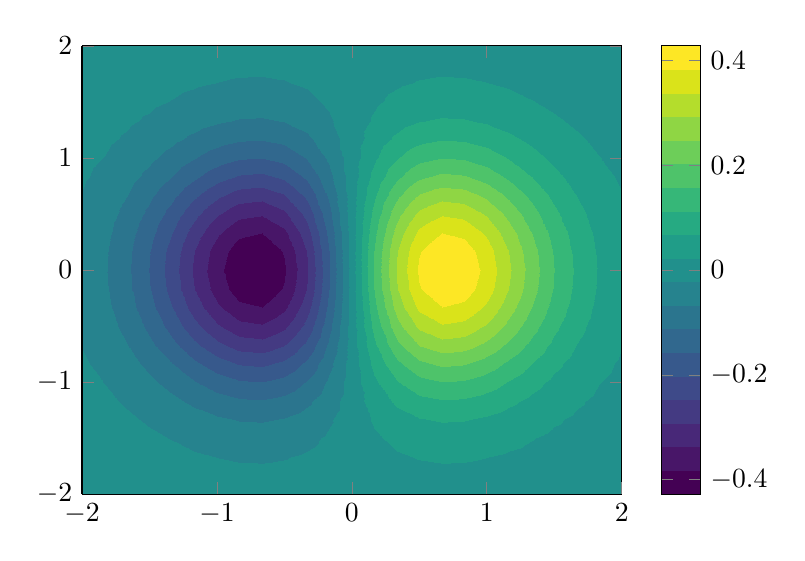
\begin{tikzpicture}
\begin{axis}[
%    title={$x \exp(-x^2-y^2)$},
    domain=-2:2, view={0}{90}, colorbar right, colormap name = viridis ]
    
  \addplot3 [contour filled={number=19,},] 
  {exp(-x^2-y^2)*x};
  
\end{axis}
\end{tikzpicture}                 % 18,12
%\pgfplotsset{compat=1.12}

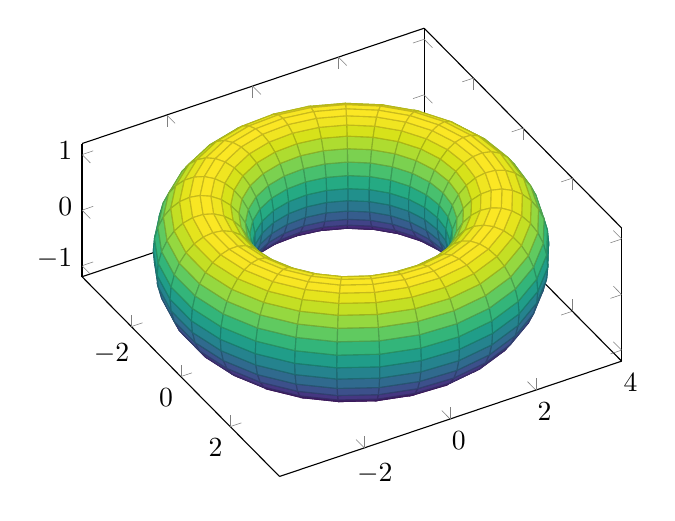
\begin{tikzpicture}
  \begin{axis}[view={60}{60}]
    \addplot3[surf, colormap/viridis, samples=30, 
              domain=0:2*pi, y domain=0:2*pi, z buffer=sort]
    ({(3+cos(deg(x)))*cos(deg(y+pi/2))}, 
     {(3+cos(deg(x)))*sin(deg(y+pi/2))}, 
     {sin(deg(x))});
  \end{axis}
\end{tikzpicture}                           % 18,12

% Drafts:
%\pgfplotsset{compat=1.12}

\begin{tikzpicture}[thick, >=stealth']
  \begin{axis}[xlabel={$x$}, ylabel={$y$}, xmin=-1.5,xmax=1.5,ymin=-1.5,ymax=+1.5, samples=17]
    \addplot3[surf, faceted color=black, fill=white, domain=-1:1, y domain=-1:1] 
      {1-x^2-y^2};
    \fill[red] (0.5,-0.5,0.5) circle (3pt);  % point is on crossing of grid lines
  \end{axis}
\end{tikzpicture}

          % 18,12

% 3rd Party examples:
%\pgfplotsset{width=18cm,height=15cm} 
%% Taken from:
% https://tex.stackexchange.com/questions/538087/how-to-plot-a-parametric-surface-helicoid-with-latex

% Looks good with aspect ratio w:h = 6:5, e.g. w=18, h=15

\pgfplotsset{compat=1.16}
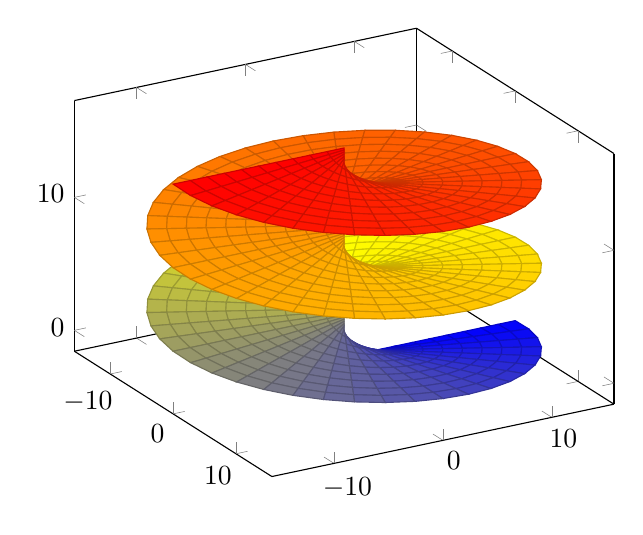
\begin{tikzpicture}
  \begin{axis}[view={60}{30}]
    \addplot3[surf, domain = 0:5*pi, samples = 101, samples y = 11, z buffer = sort]
    ({y*sin(deg(x))},
     {y*cos(deg(x))},
     {x});
  \end{axis}
\end{tikzpicture}

% Maybe try a different colormap. Maybe some sort of pastel-rainbow would look nice for this.                 % 18,15
%\include{3rdParty/TikZ_ParabolicDome}             % the width,height call seems to make no difference
%% Fancy Torus - creates memory problems - is apparently too fancy:

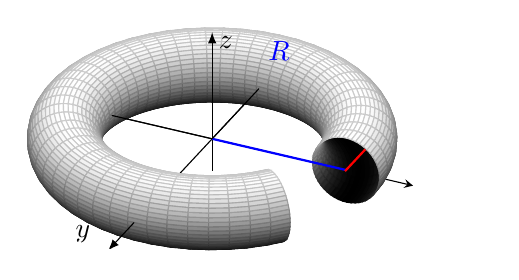
\begin{tikzpicture}
  \begin{axis}[
      axis equal image,
      axis lines=middle,
      xmax=18,zmax=5,
      ticks=none,
      clip bounding box=upper bound,
      colormap/blackwhite
    ]

    \addplot3[domain=0:360,y domain=0:320, samples=50,surf,z buffer=sort]
    ({(12 + 3 * cos(x)) * cos(y)} ,
    {(12 + 3 * cos(x)) * sin(y)},
    {3 * sin(x)});
    % use axis coordinate system to draw the radii
    \draw [thick,blue] (axis cs: 0,0,0) -- (axis cs: 12,0,0) node [midway,above=-2] {$R$};
    \draw [thick,red] (axis cs: 12,-0.2,0) -- (axis cs: 12,3.7,0) node [midway,below right=-3] {$r$};

    % use axis coordinate system to draw fake x, y and z axes
    \draw [-latex] (axis cs: 0,0,0) -- node [pos=0.9, xshift=0.5em]{$z$}(axis cs: 0,0,10);
    \draw [-latex] (axis cs: 0,-15,0) --
    node [pos=0.9, xshift=-1em, yshift=0.5em]{$y$}(axis cs: 0,-20,0);
    \draw (axis cs: 0,0,0) -- (axis cs: 0,9,0);
    \draw (axis cs: 0,0,0) -- (axis cs: -9,0,0);
  \end{axis}
\end{tikzpicture}

% from here:
% https://tikz.net/torus/
% https://github.com/janosh/tikz/
% Gives error "TeX capacity exceeded, sorry [main memory size=3000000]. \end{axis}"
% See:
% https://tex.stackexchange.com/questions/7953/how-to-expand-texs-main-memory-size-pgfplots-memory-overload
% https://www.florian-rappl.de/Articles/Page/239/latex-memory


\pgfplotsset{compat=1.14}
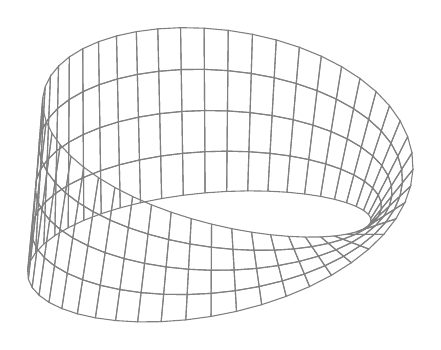
\begin{tikzpicture}
  \begin{axis}
    [
      hide axis,
      view={40}{40}
    ]
    \addplot3
    [
      surf,
      mesh, 
      shader=faceted interp,
      point meta=x,
      draw=gray,
      %colormap/blackwhite,
      samples=50,
      samples y=5,
      z buffer=sort,
      domain=0:360,
      y domain=-0.25:0.25,
    ]
    (%
      {(1+0.5*y*cos(x/2)))*cos(x)},
      {(1+0.5*y*cos(x/2)))*sin(x)},
      {0.5*y*sin(x/2)}
    );
    
%    % This is supposed to draw surface normals (I guess) - but it seems to be wrong:
%    \addplot3
%    [
%      samples=90,
%      %domain=-145:180,
%      domain=0:360,
%      samples y=0,
%      thick,
%      postaction={decorate},
%      decoration={% pgfplots manual 355-356
%        markings,
%        mark=between positions 0 and 1 step 10mm with
%        {
%          \node [single arrow, transform shape, rotate=-90, fill, draw, inner sep=0pt, single arrow head extend=1pt, text width=2.5mm, text height=0pt, anchor=west, line width=.4pt, ] {};
%        },
%      },
%    ]
%    (%
%      {cos(x)},
%      {sin(x)},
%      {0}%
%    );
    
    
  \end{axis}
\end{tikzpicture}


% See also:
% https://tex.stackexchange.com/questions/496801/moebius-strip-border
% this draws a border - which is also interesting. We want a border *and* surface normals!


% Yet another variant:
% https://tex.stackexchange.com/questions/364073/adding-lines-perpendicular-in-the-plane-to-a-mobius-band
%\begin{tikzpicture}
%\begin{axis}[
%hide axis,
%view={40}{40}
%]
%\addplot3 [
%mesh, shader=faceted interp,
%point meta=x,
%colormap/blackwhite,
%samples=100,
%samples y=5,
%z buffer=sort,
%domain=0:360,
%y domain=-0.5:0.5
%] (
%{(1+0.5*y*cos(x/2)))*cos(x)},
%{(1+0.5*y*cos(x/2)))*sin(x)},
%{0.5*y*sin(x/2)});
%
%\addplot3 [
%samples=50,
%domain=-145:180,
%samples y=0,
%thick
%] (
%{cos(x)},
%{sin(x)},
%{0});
%\end{axis}
%\end{tikzpicture}              % 18,12
% Taken from here:
% http://laberintos.itam.mx/latex-para-tesistas-ii/
% and then tweaked

\pgfplotsset{compat=1.13}

\begin{tikzpicture}

  \begin{axis}[hide axis, view={30}{50}]
  
    % backside walk, domain depends on the camera angle :-(
    \addplot3 [ultra thick, rsRed, dotted, -stealth', samples y=0,
               samples=60, domain=188:270] 
    ({(1+0.125*cos(x/2))*cos(x)},
     {(1+0.125*cos(x/2))*sin(x)},
     {0.125*sin(x/2)});

    \addplot3 [ultra thick, rsBlue, dotted, -, samples y=0,
               samples=60, domain=270:565] 
    ({(1+0.125*cos(x/2))*cos(x)},
     {(1+0.125*cos(x/2))*sin(x)},
     {0.125*sin(x/2)});


    % surface
    \addplot3 [surf, point meta=x, colormap/greenyellow, thin, line width=0.2mm, z buffer=sort, 
               samples=50, samples y=7, domain=-180:180, y domain=-0.5:0.5, opacity=0.25] 
    ({(1+0.5*y*cos(x/2))*cos(x)},
     {(1+0.5*y*cos(x/2))*sin(x)},
     {0.5*y*sin(x/2)});

    % frontside walk, domain depends on the camera angle :-(
    \addplot3 [ultra thick, rsRed, -, samples y=0, samples=60, domain=-90:188] 
    ({(1+0.125*cos(x/2))*cos(x)},
     {(1+0.125*cos(x/2))*sin(x)},
     {0.125*sin(x/2)});
     
    \addplot3 [ultra thick, rsBlue, -stealth', samples y=0, samples=60, domain=-155:-90] 
    ({(1+0.125*cos(x/2))*cos(x)},
     {(1+0.125*cos(x/2))*sin(x)},
     {0.125*sin(x/2)});     
     
     
     
  \end{axis}
  
\end{tikzpicture}              % 18,12



\end{figure}






\end{document}



\begin{comment}


Color map:
https://tex.stackexchange.com/questions/359526/defining-custom-colormap
https://tikz.dev/pgfplots/libs-colorbrewer


\end{comment}